% !TEX encoding = UTF-8 Unicode
% !TEX program = pdflatex
% !TEX spellcheck = en_US


% In order to correctly compile this document,
% execute the following commands:
% 1. pdflatex
% 2. pdflatex
% 3. pdflatex



\documentclass[amsthm,ebook]{saparticle}

% IF YOU USE PDFLATEX
\usepackage[utf8x]{inputenc}
% if you write in english and in greek
\usepackage{ucs}
\usepackage[greek,english]{babel}
\languageattribute{greek}{polutoniko}

% IF YOU USE XELATEX
%\usepackage{polyglossia}
% if you write in italian
%\setmainlanguage{italian}
% If you want put some ancient greek:
%\setotherlanguage[variant=polytonic]{greek}
%\newfontfamily{\greekfont}[Ligatures=TeX]{Palatino Linotype}

% dummy text (remove in a normal thesis)
% remove if not necessary
\usepackage{siunitx}
%Natbib for bibliography management
\usepackage[authoryear]{natbib}
% custom commands
\newcommand{\bs}{\textbackslash}

%%%%%%%%
%TITLE:%
%%%%%%%%

%all title info missing!
\title{A VIRTUAL RESEARCH ENVIRONMENT TO DOCUMENT AND ANALYZE NON-ALPHABETIC WRITING SYSTEMS. A Case Study for Maya Writing.}
\author[bonn]{Katja Diederichs\corref{first}}
\author[bonn]{Sven Gronemeyer}
\author[bonn]{Christian Prager}
\author[bonn]{Elisabeth Wagner}
\author[bonn]{Franziska Diehr}
\author[bonn]{Brodhun Maximilian}
\author[bonn]{Nikolai Grube}

\address[bonn]{missing}

\cortext[bonn]{missing} 

\begin{document}

\maketitle

\begin{abstract}
No existing digital work environment can sufficiently represent the traditional epigraphic workflow `documentation,
analysis, interpretation, publication' for a non-alphabetic writing system. Using the Maya hieroglyphic script, this
workflow will be transferred to a digital epigraphy. Digital methods and tools will be developed and reused in a
Virtual Research Environment to create a freely accessible, annotated textual corpus, including metadata on cultural
and object history and references.
\end{abstract}
\keywords{Classic Mayan, Digital Epigraphy, TEI, EpiDoc, CIDOC-CRM, Metadata Schema, Open Science}







\section{Digitalizing the Epigraphic Workflow}


\noindent In order to develop a digital work environment that represents the traditional epigraphic workflow for documenting and
studying inscriptions in a non-alphabetic script, the individual steps of this workflow need to be technically
implemented using methods and tools from the Digital Humanities. The workflow begins with the documentation of the text
carriers and compilation of descriptive data; proceeds to epigraphic analysis, including sign classification and
transliteration and transcription of the texts; continues with morphological segmentation and linguistic
interpretation; and concludes with translation and digital publication of the inscription \citep{Diederichs2015}. 

The Virtual Research Environment (VRE) TextGrid initially provides the necessary framework for executing the workflow
that technically facilitates documentation and digital registration of the text carriers in the form of images and
drawings, as well as annotation of the objects with metadata. TextGrid offers input forms, annotation tools, and a
Text-Image-Link-Editor, and provides long-term storage, and free access to the data in an open web repository \citep{NeurothLohmeier2011}. 

Although more detailed steps in an epigraphic workflow, such as detailed linguistic and epigraphic analysis of primary
texts, can be technically carried out within a VRE such as TextGrid, they still necessitate creation and adaptation of
their own XML-based metadata model, as well as annotation schemas for object and textual contexts \citep{Prager2015}. Using
this approach, the Maya hieroglyphic script will for the first time be able to fulfill a central requirement of corpus
linguistics, namely machine readability \citep{McEneryWilson2001}. 

Fig.~\ref{fig:1} provides a schematic illustration of the following points that represents in great detail the steps in
epigraphically analyzing Maya inscriptions, a process which can also be used in modified form to study other
non-alphabetic writing systems. The modulated VRE is thus applicable not only to the study of Maya texts, but also to
researching texts composed in other hieroglyphic, cuneiform, or linear writing systems. 




\begin{enumerate}
\item Identification of hieroglyph blocks by alphanumeric classification 
\item Original spelling
\item Reading order of individual signs 
\item Number of signs within one block 
\item Identification and isolation of signs in one block 
\item Classification of signs based on the sign catalog of Eric Thompson \citep{Thompson1962}
\item Classification of signs in one block \citep{Thompson1962} 
\item Transliteration of individual signs 
\item Description of sign function (syllables, logographs)
\item Transliteration 
\item Broad transcription
\item Morphological segmentation 
\item Morphological analysis 
\item Determining congruence between block- and word-boundaries 
\item Determining syntactic function 
\item Determining sentence constituents 
\item Translation of single words 
\item Literal translation 
\item Rough translation
\end{enumerate}



\begin{figure}[!bp]
\centering
 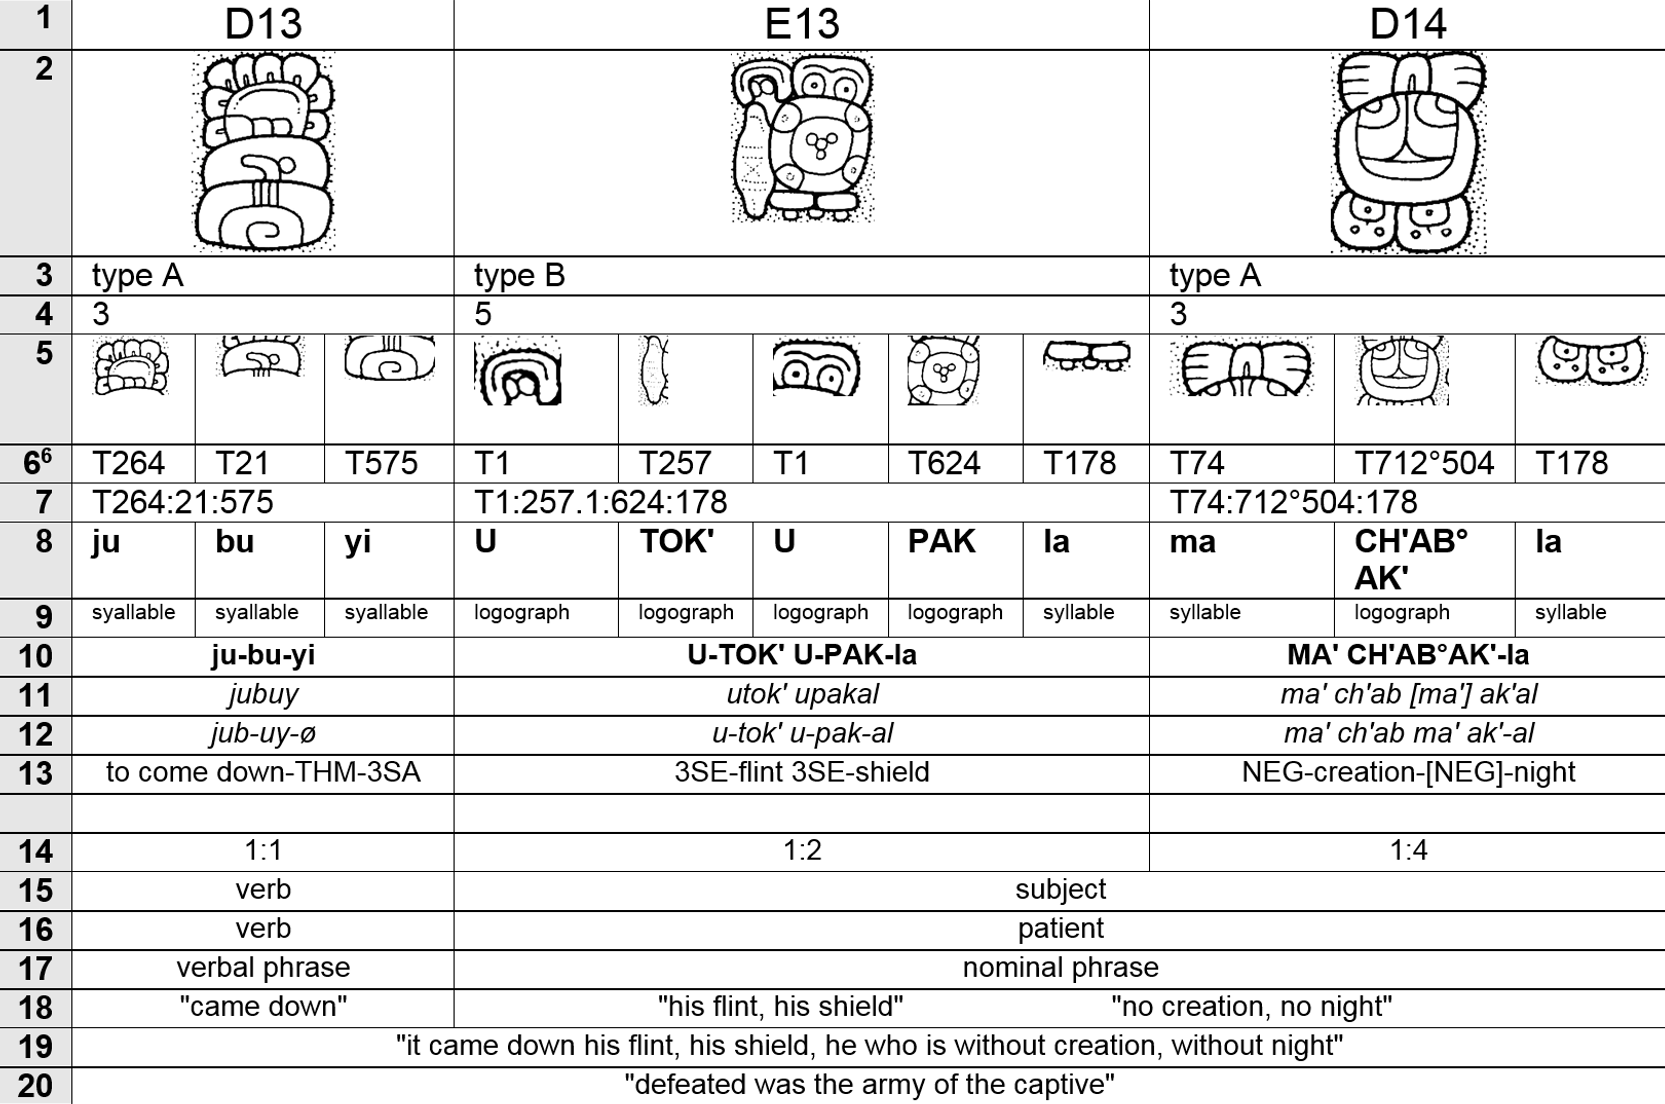
\includegraphics[width=\columnwidth]{EAGLE2016submission8revisedx-img001.png}
\caption{Visualization of the important steps in the workflow of epigraphic analysis, drawings by \citet{Prager2015}}
\label{fig:1}
\end{figure}





\subsection[Conceptual Questions]{Conceptual Questions}
When developing and technically implementing the digital epigraphic research environment, the major focus is on pursuing
the following objectives: 
\begin{enumerate}
\item creation of a markup schema to represent these steps (which in practice are interconnected
and may also occur parallel to each other in the form of alternative interpretations); 
\item defining of the precise requirements that a data structure must fulfill in order to sufficiently represent complex
i.e. non-alphabetic textual data for epigraphic analysis and research. 
\end{enumerate}


\section[Prerequisites for Making a Non{}-Alphabetic Writing System Digitally Accessible]{Prerequisites for
Making a Non-Alphabetic Writing System Digitally Accessible}
\noindent In order to make syllabic or logo-syllabic writing systems accessible for corpus linguistics, for instance to carry out
a corpus analysis as part of the basic lexicography required to compile a dictionary of Classic Mayan, the phonology,
morphology, syntax, semantics, and pragmatics of the language in question must be captured, marked up, and saved in the
corpus. As such, the basic characteristics that distinguish the graphematic lexicon of syllabic and logo-syllabic
scripts from those of alphabetic writing systems must be taken into account. Thus, methodological and technical
prerequisites must be fulfilled in order to be able to digitally represent and analyze a non-alphabetic script, such as
Classic Mayan, for the purposes of epigraphic analysis.

\subsection[Registering Object Data ]{Registering Object Data}
\noindent When designing the digital epigraphic work environment, one must also account for the current state of decipherment of
the script and language that are to be documented. Thus, Classic Mayan presents great challenges, as at least one third
of the known graphemes have not yet been completely deciphered. Even when a lexeme can be read, its etymology or
semantic domain is often unknown, and in some cases not even its lexical class can be determined, which causes
difficulties when attempting to read and understand a text. In order to decode an unknown sign, word, or sign sequence
in its respective context of use, for instance, semantic fields are generally investigated by means of applied
substitution. From a structuralist perspective, this method investigates the paradigmatic relation between two
linguistic entities as indicated by whether or not they appear in the same context \citep{Bussmann2002}. This step yields
results when sufficient quantities of data can be digitally compiled, marked up and investigated using corpus
linguistics. 

The VRE currently being planned is the laboratory for this process, where new decipherments will be obtained and
existing readings will be tested against primary source material while also considering all of the contextual data. The
context of the contents that is referenced during decipherment may refer to the text carrier itself. For this reason,
registering data on the object on which the text is written is just as important as documenting the text itself. 

The decoding of Ugaritic cuneiform at the beginning of the twentieth century provides an example of a successful
decipherment that resulted from studying the relationship between object and textual data. Scholars suspected that the
word ``axe'' occurred in repeating, brief sign sequences on inscribed bronze axes. Building on this hypothesis, they
determined the phonetic values of individual signs using data on the Canaantic language and completely deciphered the
script \citep{Day2002}. Such investigations enable initial association of signs with both content and function in the
relevant language so that the signs may later be grammatically, morphologically, semantically, etc., defined and
eventually deciphered. This work also facilitates more precise typological classification of a writing system
\citep{Gronemeyer2015}.

Like the relationship between writing and the object, the relationship between text and image must also be coded.
Associated depictions can potentially illuminate the contents of an inscription. Working from this analytical basis, a
writing system can be registered in its respective contexts of use in order to derive semantic meanings and, ideally,
linguistic decipherments. As such, contextual information concerning the text carrier as an object must be recorded,
because its physical features may influence the text’s contents and arrangement. In this respect, the size of the
object, for example, may be just as influential as the material itself.

For example, the text carrier may influence scribal economy. The recent discovery of an inscription on very hard jade in
Nim Li Punit (Belize) illustrates how the use of this particular writing surface can lead to a reduced spelling,
meaning that the scribe omitted final syllables or used very simple sign variants that were almost geometric. 

The form of a text carrier and its function also influence the text. Different lexemes may thus be determined for
describing round or quadrilateral altars, with the result that conclusions may be drawn concerning the semantics and
possible linguistic decipherments. Physical description of the text carrier as an object and its linguistic,
historical, and cultural contextualization are indispensable for deciphering a previously unknown text or analyzing its
arrangement. These metadata must be consulted in order to grammatologically and linguistically analyze the text’s
contents. 

Modelling an object biography and culturally contextualizing the texts must be initially addressed with information
technology in order to facilitate epigraphic analysis of the text’s contents in its extra-linguistic, cultural context.
Thus, it is necessary to create an object metadata schema that captures such information concerning the language’s
cultural area and makes it available for use. 

For these purposes, an epigraphic object metadata schema that compiles and represents extra-linguistic information about
the inscriptions in an ontological structure must be created, in addition to an XML-based analytical metadata schema
for linguistics. 

The CIDOC-CRM standard for documenting cultural heritage offers a broad foundation that can be supplemented with other
standards, such as Dublin Core or the SKOS vocabulary. In addition to taking advantage of the comprehensive
understandability of CIDOC-CRM, the scheme also requires to reuse data and to connect them with data from other
research projects in the spirit of Linked Open Data \citep{Diederichs2015, Prager2015}. %corrected from Prager 2014, not in biblio

\subsection[Making Linguistic Data Accessible]{Making Linguistic Data Accessible}
\noindent An interdisciplinary and widely accepted standard that takes into account both generalized and special characteristics
of writing systems beyond those of a single script must be developed in order to be able to satisfactorily annotate
records from various writing traditions that use syllabic signs and logograms to represent language.

In most cases, the scripts annotated and encoded in TEI and also those prepared for epigraphic analysis in EpiDoc are
alphabetic, and most of them are linear and arranged in rows. Non-alphabetic writing systems, such as Egyptian, various
cuneiform systems, or Hieroglyphic Luwian, arrange their graphemes principally in groups or blocks, and only
secondarily in rows or columns, with a high rate of metathesis \citep{Lacau1903} in order to optimize the use of space.
Furthermore, many of these writing systems demonstrate a high degree of allography, which is no longer apparent in a
pure transliteration. Various desiderata become apparent when an epigraphic project attempts to use the standards
provided by TEI and EpiDoc to edit texts composed in these scripts. 

Annotating texts composed in such writing systems that use only alphabetic transcription is insufficient; instead, the
original spelling of a lemma should be represented. This approach facilitates studies of paleography or sign usage
across time and space. In addition, it can reveal preferred sign arrangements within a block or preferences for
particular signs that correspond to the material used or to the subject of the text, for instance.

Thus, when creating a standard for non-alphabetic scripts, object metadata and annotations for orthographic and
linguistic analysis must be taken into account, and the creative process should also promote discussion of
terminological and typographic conventions for these annotations \citep{SachseDurr2015}. The goal is to create a generic
markup model that can be implemented regardless of the particular script or language in question. The inscriptions of
the Maya hieroglyphic writing system alone feature attestations of various vernacular languages \citep{LacadenaWichmann2002}, a phenomenon which raises several preliminary questions: what exactly are the demands, and what are the goals of
an epigraphic and linguistic annotation? Where do possibilities and limitations exist for annotating these writing
systems using established standards, such as TEI or EpiDoc? Existing standards have to be modified to some extend and
possibly new standards have to be created, to overcome these limitations. 




\subsubsection[Representing the Primary Text Source]{Representing the Primary Text Source}
When defining a text, acknowledging an interpretation of the source text itself is unavoidable. The meaning of the
``original text'' that resides in the ``source text'' is an important point of discussion in epigraphy. Thus, the
annotation does not contain a guiding text in the conventional sense, because it is merely reconstructed using all
given text information and one’s own conclusions and interpretations, and then represented with the aid of alphabetic
transliteration and transcription. In this respect, one should always leave open the possibility of separating primary
data (in the case of hieroglyphic texts, photographs of the text carriers, for example) and secondary data (e.g.
drawings or interpretive annotations) \citep{Stuhrenberg2012}. This strategy can be implemented using stand-off annotations
for data. Similarly, such an annotation should permit multiple descriptions, i.e. alternative statements concerning the
data \citep{Stuhrenberg2012}. For example, sign sequences in Classic Mayan can be variously analyzed depending in a
particular vernacular context \citep{Gronemeyer2014}. Only in this manner can various ways of thinking be appropriately
recorded and relayed to the scientific community for discussion. 

A key objective of the XML-based markup of hieroglyphic, cuneiform, or linear texts should thus be to represent the
original spelling and arrangement of the signs in their respective contexts. A linear transcription alone cannot
represent the original text or primary source in its entirety, as many details remain undocumented. For example, signs
in Maya hieroglyphic texts are not arranged according to their literal reading order, but instead in spatially
distinct, square or rectangular units (so-called ``blocks''), each of which in most cases corresponds to a word or
morpheme sequence. A detailed markup of the original text is therefore of great importance, particularly for partially
deciphered and undeciphered graphemes and writing systems in general. In such cases, an alphanumerical or numerical
nomenclature is often used to refer to the signs in order to carry out a corpus linguistic analysis of the texts. The
arrangement of each block, as well as the text and its position on a text carrier, should be documented as well. To
fully understand a writing system – i.e. the language and information expressed in it - a detailed representation of
the primary source and its context must be a key objective in the digital markup of documents. When studying complex
writing systems (respectively non-alphabetic writing systems), digital documentation of the original spelling using
annotation standards like TEI is a basic prerequisite for conducting a detailed graphemic and graphetic analysis of the
relevant script and for providing a basis for a linguistic and corpus linguistic investigation. This need represents a
significant desideratum in epigraphic research, and it also constitutes a core pillar of computational linguistics
\citep{McEneryWilson2001}. 

In an interdisciplinary effort, epigraphers and experts of digital markup-languages alike need to discuss methods for
investigating syllabic and logo-syllabic writing systems using the XML-based standards like TEI or EpiDoc. When doing
so, they should discuss the following points of emphasis, among others: 




\subsubsection[Graphetics ]{Graphetics }
Graphetics concerns the formal structure of linguistic units and the structure of texts \citep{Crystal1997}. Classic Maya
hieroglyphic inscriptions, for instance, may display a very high degree of variation in writing styles for arranging
texts, a phenomenon which is deserving of investigation. In this manner, various systems of notation are studied in
their individual, social, and typographic aspects, for instance \citep{Bussmann2002}. Similarly, in paleography, script
decipherment is examined from graphetic perspective \citep{Bussmann2002}. The arrangement of texts, for instance, different
grapheme or block sizes of text fields, or different styles of hieroglyphic writing (equivalent to alphabetic font
style and size) are analyzed. 

Research addresses the degree to which attested variation in the composition of hieroglyphic texts may be ascribed to
specific scribal schools or to regional forms of expression, rather than to differences in the meaning of the signs’
contents. 




\subsubsection{Graphemics }
When analyzing the contents of these texts, it is important to investigate meaningful variation underlying the manner in
which the writing is arranged and to thereby identify distinct units \citep{Bussmann2002}. Graphemics is devoted to this area
of research, and consequently to exploring the meaningfully distinct features of signs. 




\subsubsection[1. Allography of Graphemes ]{1. Allography of Graphemes }
% THESE ARE SUBSUB*SUB*SECTIONS...
A very important example of a subject of graphemic research is provided by allography, a phenomenon which describes a
1:n relationship between a grapheme and its various graph representations \citep{Crystal1997}. 

The process of establishing a suitable annotating-tool thus must be oriented toward a series of questions: What is the
significance of allography for the respective grapheme inventories? Are allographs annotated in the transliteration or
transcription of the respective writing systems? 

For example, in Maya writing, there are over twenty different allographs for the vowel sign {\textless}u{\textgreater},
which is used e.g. as the 3rd person ergative pronoun u- ``he, she, it''. Additional research questions may comprise 1)
the reading order of the signs in context; 2) the existence of word separators or other graphic aids used to
differentiate between meaningful units or words; 3) multiple possibilities for establishing a reading order of signs
within a block that are equally meaningful (with alternatives documented or marked by epigraphers); 4) the reading
order of meaningful units within the texts; 5) variations or violations of these orders (and if so, with a markup as
well); 6) cases where images appear with the text and their possible relation; 7) integration of texts into the images
or vice versa.
%what to do with this lists? another below.



\subsubsection[2. Graphotactic Strategies of a Writing System ]{2. Graphotactic Strategies of a Writing System
}
For analysis, it is important to convey the graphemics of a writing system, which are lost in an alphabetic
transliteration. Graphemics concerns sign function, or graphotactic strategies for constituting a meaningful unit or
word. Representing the reading order of signs in the text and in each block is similarly imperative. To
graphotactically link individual signs in a hieroglyphic block in Maya writing, various representational rules may be
used (see Fig.~\ref{fig:2}), e.g. affixation, infixation, conflation, or superimposition \citep{Zender1999}. Additional typical,
functional traits of logo-syllabic writing systems include underspellings, diacritics, phonemic complements and
indicators, semantic classifiers and determinatives, and sign class convergences. However, these characteristics may
have very diverse graphotactical manifestations in different writing systems, which nonetheless need to be standardized
and communicated in a digital structure in order that researchers may thus take note of various interpretations under
discussion. 

\begin{figure}[!bp]
\centering
 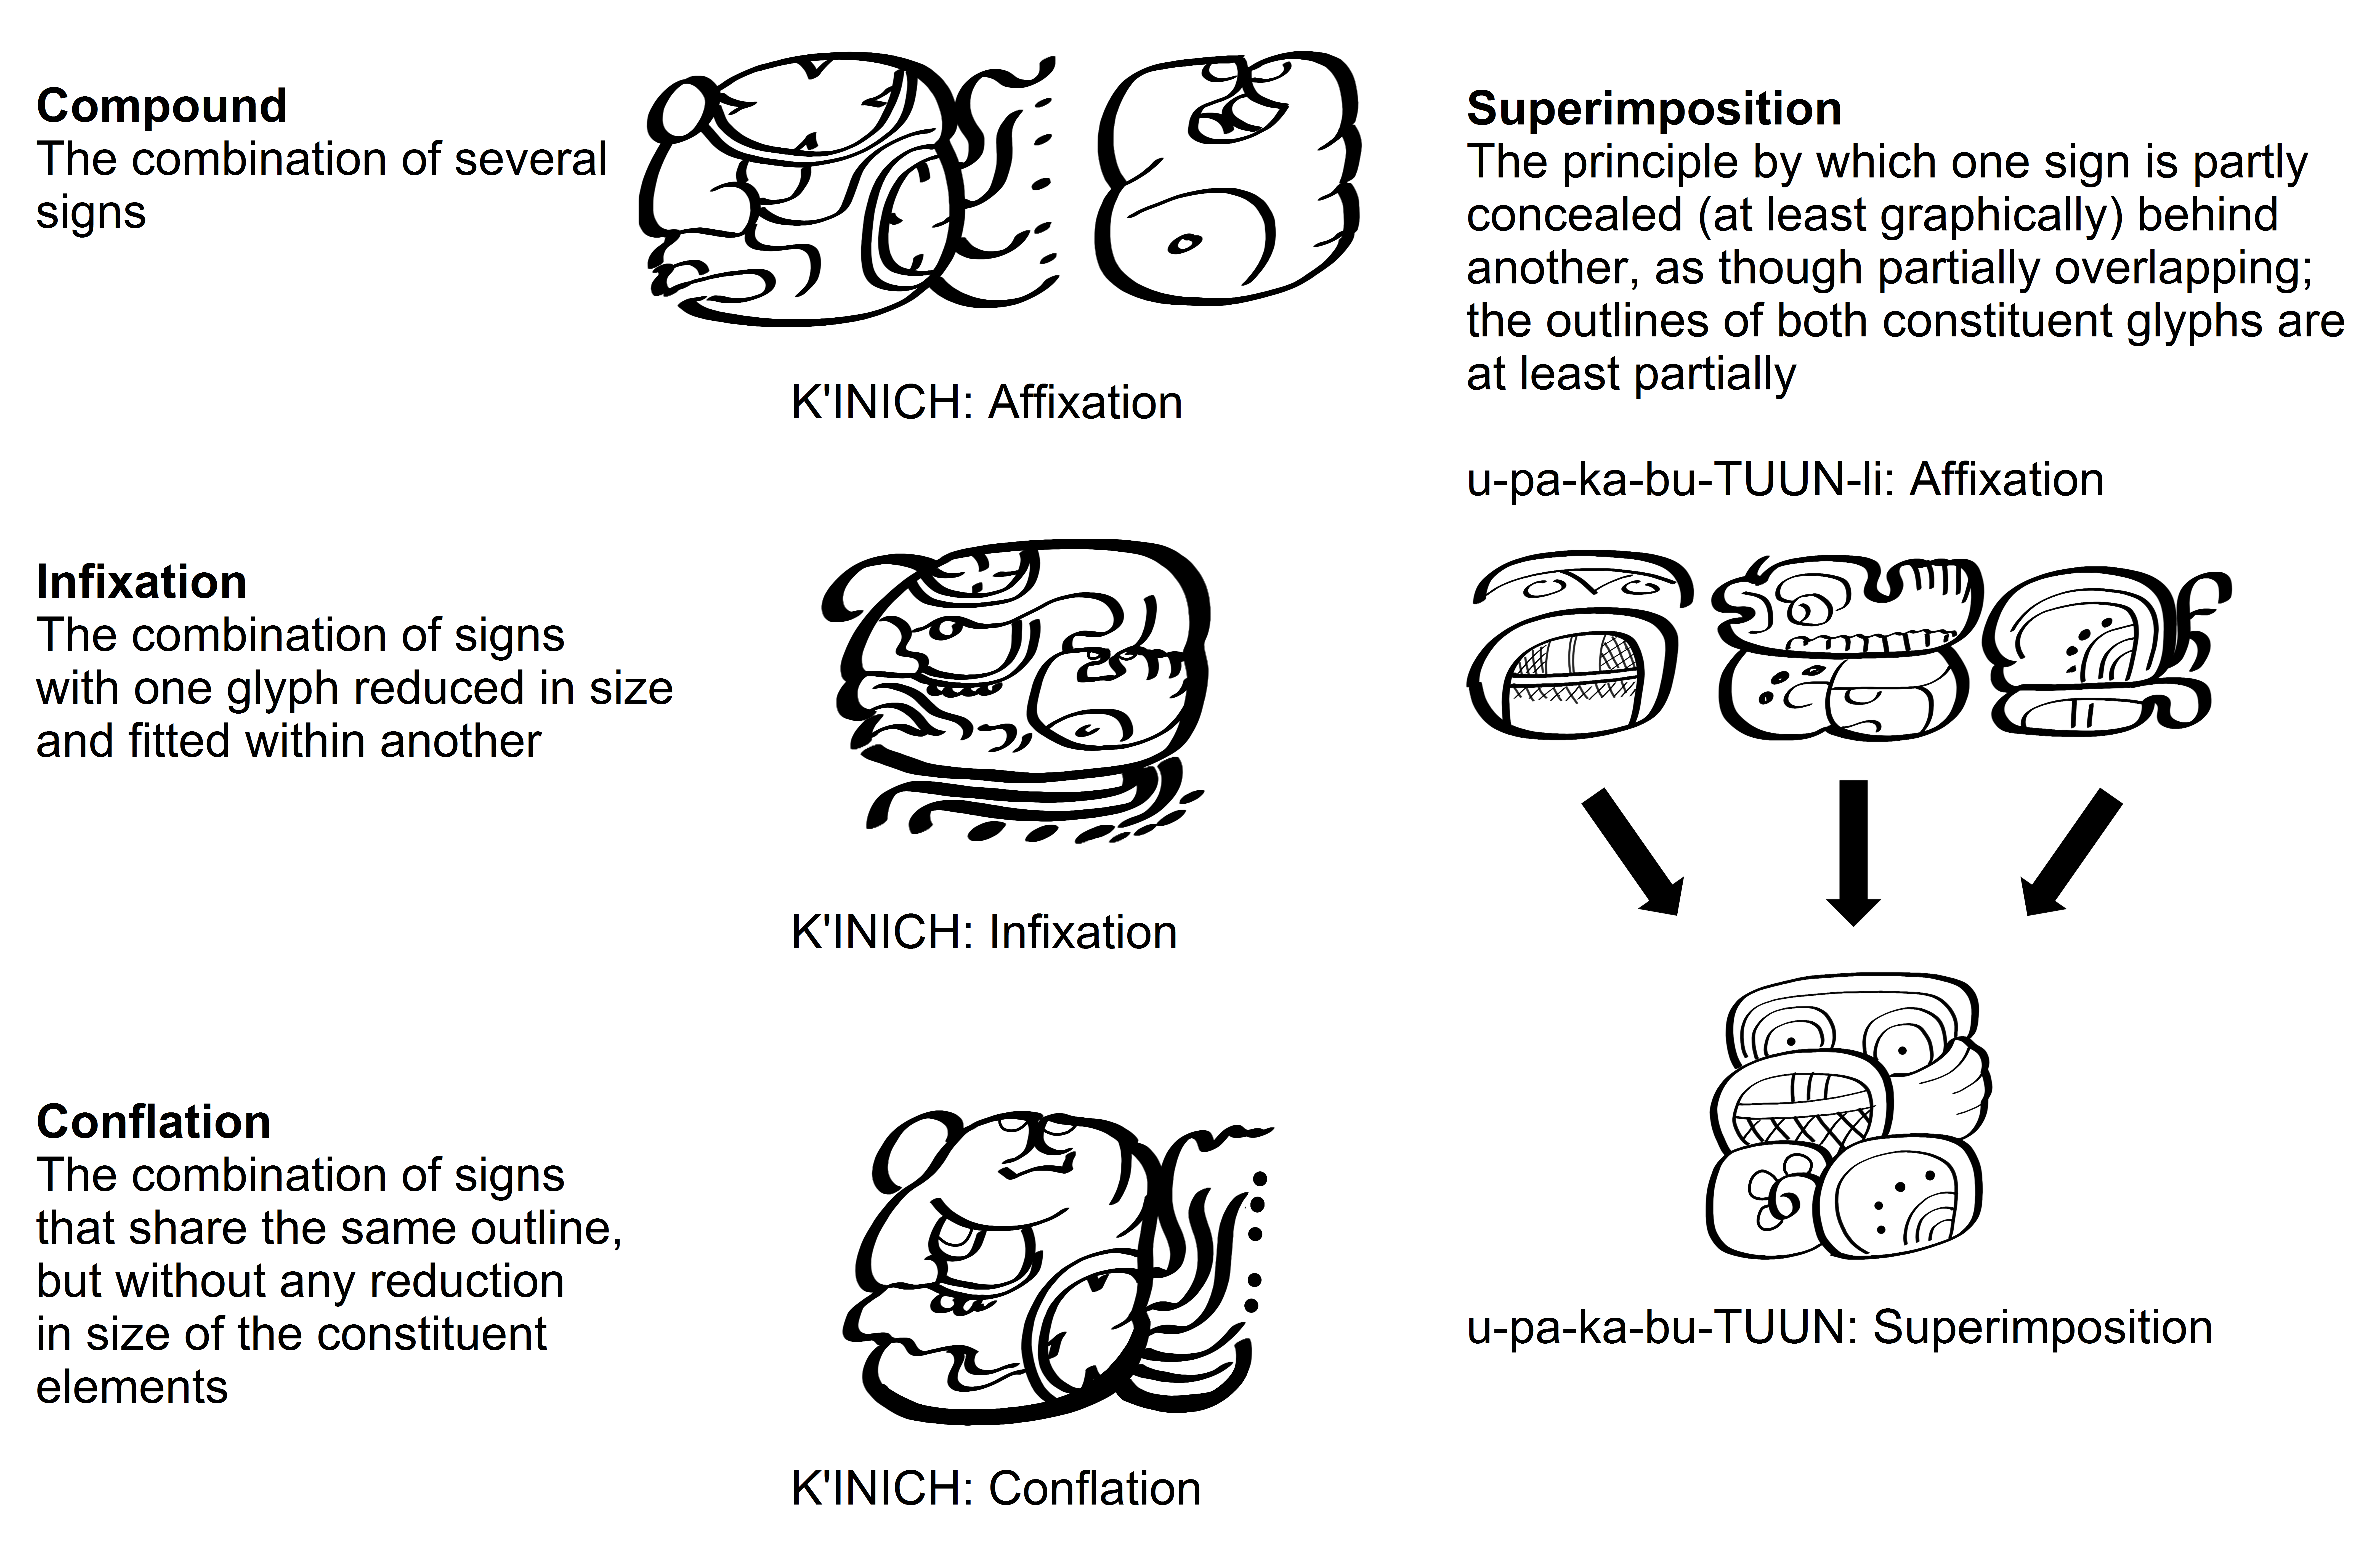
\includegraphics[width=\columnwidth]{EAGLE2016submission8revisedx-img002.png}
\caption[Some possible sign combinations in Classical Mayan hieroglyphs after \citet{Zender1999}, drawings by
\citet{Prager2015}]{Fig. 1.2. Some possible sign combinations in Classical Mayan hieroglyphs after \citet{Zender1999}, drawings by \citet{Prager2015}}
\label{fig:2}
\end{figure}


\subsubsection[Signary: Sign Classification and Sign Catalogs ]{Signary: Sign Classification and Sign Catalogs }
\noindent The graphemic lexicon provides a central reference for marking up texts composed in non-alphabetic writing systems. In
the case of the Maya script, signs whose phonemic reading is unknown or unconfirmed are denoted using reference systems
from various classification catalogues \citep[e.g.]{Thompson1962}. Use of question marks for indicating unclear readings, for
example, should be avoided, because such signs impair machine readability and sometimes represent control characters or
part of an escape sequence. In this context, it should be determined what significance sign classifications and
nomenclatures have in their respective branches of epigraphic research. Also their role in transliterating and
transcribing texts in the respective writing system, as well as in sign classification is to be examined. Sign
inventories constitute a central authority in an epigraphic VRE, and they need to be modified or supplemented in
accordance with the ever-changing state of research as soon as newly discovered material is entered and signs are
identified that had not previously been isolated or identified as discrete graphemes. 

\subsubsection[The State of Decipherment and the Readability of Texts ]{The State of Decipherment
and the Readability of Texts }
\noindent In the case of unreadable or only partially deciphered writing systems, the question in the forefront is the state of
decipherment of the relevant writing system and the handling of undeciphered signs or text passages. As archaeological
artifacts, texts are also subject to processes of decay that inhibit visible legibility. It has several implications:
1) the treatment of undeciphered signs or text passages; 2) the indication of physical gaps (as texts are also subject
to processes of decay that inhibit visible legibility) and their marking in the transliteration and transcription of
the text; 3) the treatment of hypothetical, yet plausible, readings of singular signs or passages; 4) the handling of
alternative readings of the same passage; and 5) a review to what extent the EpiDoc Metadata standard, into which the
Leiden Conventions have also been incorporated, is able to capture these features of readability and alternative
interpretations of inscriptions.

These and other characteristics of non-alphabetic scripts, which to a certain extent reach beyond the epigraphic
problematic of alphabetic writing systems, illuminate a desideratum here and the need to formulate ideas that
contribute to the design and modelling of appropriate XML-based metadata schemas. 




\section{Open Science Strategy}
 

\noindent A Digital Humanities project working in the spirit of Open Science fundamentally intends the work environment that it
develops to be reused. As such, a VRE for non-alphabetic writing system such as that of the Classic Maya should be
developed as generically as possible, in order that structural interoperability may ensure that they can be reused by
similar epigraphic projects.

In this respect, any metadata schema that is created should be widely intelligible and ensure the data’s syntactic and
semantic interoperability by using common, given, XML-based annotation and metadata standards, like TEI and EpiDoc, and
controlled vocabularies, such as SKOS, that are already established in the Digital Humanities \citep{Diederichs2015}.

Another objective of database projects in the Digital Humanities should be to ensure open access to their data and
metadata, and thus to maximize usage of their research by maximizing user access to it. As all current and future
research and innovation stands on the shoulder of giants, an efficient system for broadly disseminating and allowing
uninhibited access to the project’s research (raw data and metadata), as well as for guaranteeing the contents’
productive reuse, must be ensured through the use of free licenses \citep{DFG2014}. 

As such, all the contents of a database and data infrastructure that are being planned will be made available under
so-called ``Open'' licenses (Open Access, Open Source, Open Methodology, Open Data, etc.), with the goal of pursuing a
comprehensive Open Science strategy \citep{Diederichs2015}. 

All methods and the process of developing tools must thus be carefully documented to maximize reuse of all schemas and
software. In particular, all research information and results should be made available not only to the scientific
community, but also to the general public, to contribute to the digital safeguard and dissemination of humanity’s
cultural heritage. 




\section[Summary ]{Summary}
\noindent The creation of digital infrastructures and metadata schemas that facilitate recording and further analysis of the
appropriate annotation for non-alphabetic writing systems, including their respective cultural contexts, is a
desideratum in the Digital Humanities that needs to be addressed.

The recommendations articulated here for an object database, as well as for a structure for recording epigraphic and
linguistic data, can make a significant contribution to understanding how traditional epigraphy can be transferred to
digital form. In working towards this goal, methods and tools from the field of Digital Humanities will be suitably
adapted to the needs of epigraphy, and new methods and structures from the digital world will find their way into
digital epigraphy. 

\nocite{Gronemeyer2014}

\bibliographystyle{sapauth-eng}
\bibliography{../../EAGLE}

\end{document}
